\chapter{Automatic Differentiation}
\label{chap:autograd}


\begin{figure}[!ht]
    \centering
    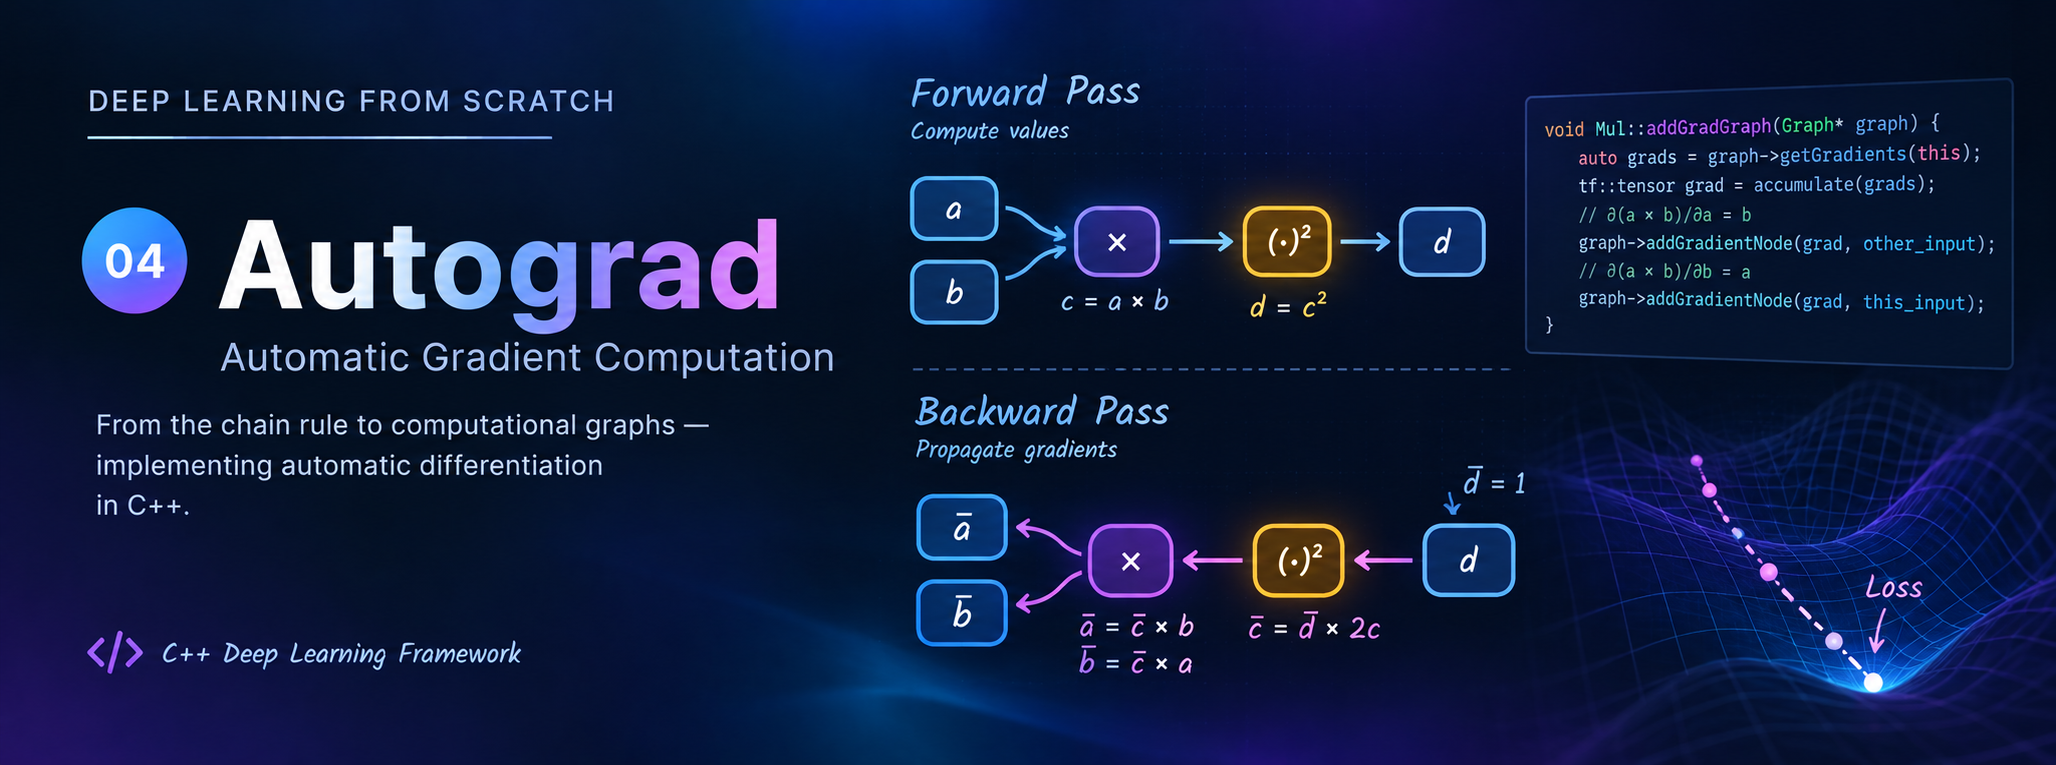
\includegraphics[width=\textwidth]{../../images/05_Autograd_ Forward and Backward Passes.png}
\end{figure}


\section{Autograd 101}

Automatic gradient computation, commonly called \emph{automatic differentiation} or \emph{autodiff}, is a technique for calculating derivatives of a computation with respect to its inputs and parameters.

Consider the function

\[
y = x^2 + 3x.
\]

Its derivative with respect to \(x\) is

\[
\frac{dy}{dx} = 2x + 3.
\]

For a simple expression, deriving the derivative manually is straightforward. However, neural networks can contain many tensor operations distributed across multiple layers. Manually deriving and implementing every possible derivative for every possible model would quickly become impractical.

Automatic differentiation addresses this problem by applying derivative rules to the operations performed during a computation and combining them using the chain rule.

It is important to distinguish autodiff from symbolic differentiation and numerical differentiation. Symbolic differentiation manipulates mathematical expressions to produce derivative expressions, while numerical differentiation estimates derivatives using numerical approximations, such as finite differences. Automatic differentiation instead propagates derivative information through the computation itself.

\section{Forward Propagation and Backward Propagation}

Consider a small example:

\[
a = 2,\qquad b = 3,
\]
\[
c = a+b,\qquad d = c^2.
\]

During the forward pass, the intermediate and final values are calculated:

\[
c = 5,\qquad d = 25.
\]

Suppose we want to calculate the derivatives of \(d\) with respect to \(a\) and \(b\). Applying the chain rule gives

\[
\frac{\partial d}{\partial c} = 2c = 10.
\]

Since \(c=a+b\),

\[
\frac{\partial c}{\partial a}=1,
\qquad
\frac{\partial c}{\partial b}=1.
\]

Therefore,

\[
\frac{\partial d}{\partial a}=10,
\qquad
\frac{\partial d}{\partial b}=10.
\]

The forward pass calculates the values of the computation, while the backward pass calculates how changes in those values influence the selected output.

This distinction is fundamental to training neural networks: the forward pass produces predictions and the backward pass computes the gradients needed to update trainable parameters.

\section{Why Reverse-Mode Automatic Differentiation?}

Automatic differentiation can be performed in different modes. Two commonly discussed approaches are forward-mode and reverse-mode differentiation.

\begin{itemize}
    \item \textbf{Forward mode} propagates derivative information alongside the forward computation.
    \item \textbf{Reverse mode} first evaluates the computation and then propagates gradients backward from the output.
\end{itemize}

Reverse mode is especially useful when a function has many inputs but relatively few outputs. Neural networks often have a large number of trainable parameters and a scalar loss, making reverse-mode differentiation a natural choice for computing the gradients required during training.

LearnDeep builds on its graph-mode execution to support this process. Since the forward operations and their dependencies are recorded in a computational graph, the framework can traverse those dependencies in reverse order and construct the corresponding gradient computation.

\section{Constructing the Gradient Graph}

The autodiff implementation in LearnDeep follows three broad steps:

\begin{enumerate}
    \item \textbf{Recording dependencies:} operations establish relationships between their input and output tensors in the computational graph.
    \item \textbf{Propagating gradients:} starting from the selected output, the framework visits operations in reverse dependency order and applies the derivative rule associated with each operation.
    \item \textbf{Accumulating gradients:} when a tensor contributes to multiple downstream operations, the gradient contributions from those paths must be added together.
\end{enumerate}

Each operation is responsible for registering the backward computation corresponding to its derivative rule. In LearnDeep, this responsibility is represented by an \texttt{addGradGraph()} routine that receives a pointer to the gradient graph.

The following simplified pseudocode illustrates the idea for a multiplication operation:

\begin{lstlisting}[
    language=C++,
    caption={Conceptual gradient-graph construction for multiplication},
    label={lst:mul-add-grad-graph}
]
void Mul::addGradGraph(Graph* graph) {
    // Retrieve gradients arriving from downstream operations.
    std::vector<tf::tensor> incoming_gradients =
        graph->getGradients(this);

    // Accumulate incoming gradients where necessary.
    // ...

    // For z = a * b:
    // dz/da = b
    // dz/db = a

    // Register backward operations that multiply the
    // incoming gradient by the opposite input.
    // ...

    // Store the resulting gradient nodes for each input.
}
\end{lstlisting}

The example is intentionally simplified. It illustrates the responsibilities of the routine rather than specifying the complete implementation or its ownership details.

For a multiplication \(z=ab\), the local derivatives are

\[
\frac{\partial z}{\partial a}=b,
\qquad
\frac{\partial z}{\partial b}=a.
\]

If the incoming gradient from downstream computation is \(\bar{z}\), the gradients propagated to the inputs are

\[
\bar{a}=\bar{z}b,
\qquad
\bar{b}=\bar{z}a.
\]

Here, the bar notation represents the gradient propagated to a tensor. In a computational graph with multiple downstream paths, these contributions must be accumulated before the gradient is propagated further upstream.

This is how the framework builds the backward computation associated with each supported operation.

\section{Visualizing the Forward and Backward Graphs}

Consider the computation

\[
c = a b,
\qquad
d = c^2.
\]

The forward graph describes how the output is calculated from the inputs:

\begin{center}
\begin{tikzpicture}[
    node distance=1.5cm,
    every node/.style={draw, rounded corners, align=center, minimum width=1.5cm, minimum height=0.7cm},
    >=stealth
]
\node (a) {\(a\)};
\node[right=1.4cm of a] (mul) {Multiply};
\node[above=0.9cm of mul] (b) {\(b\)};
\node[right=1.4cm of mul] (c) {\(c=ab\)};
\node[right=1.4cm of c] (sq) {Square};
\node[right=1.4cm of sq] (d) {\(d=c^2\)};
\draw[->] (a) -- (mul);
\draw[->] (b) -- (mul);
\draw[->] (mul) -- (c);
\draw[->] (c) -- (sq);
\draw[->] (sq) -- (d);
\end{tikzpicture}
\end{center}

The graph begins with the inputs \(a\) and \(b\). Multiplication produces \(c\), which is then squared to produce \(d\).

For reverse-mode differentiation, we seed the output gradient with

\[
\bar{d}=\frac{\partial d}{\partial d}=1.
\]

For the square operation,

\[
\bar{c}=\bar{d}\,2c.
\]

For the multiplication operation,

\[
\bar{a}=\bar{c}b,
\qquad
\bar{b}=\bar{c}a.
\]

The backward computation therefore follows the derivative rules of the forward operations, rather than simply repeating the original operations in reverse order.

\begin{center}
\begin{tikzpicture}[
    node distance=1.3cm,
    every node/.style={draw, rounded corners, align=center, minimum width=1.8cm, minimum height=0.7cm},
    >=stealth
]
\node (gd) {\(\bar{d}=1\)};
\node[below=of gd] (sqgrad) {Multiply by \(2c\)};
\node[below=of sqgrad] (gc) {\(\bar{c}\)};
\node[below left=1.0cm and 0.7cm of gc] (gaop) {Multiply by \(b\)};
\node[below right=1.0cm and 0.7cm of gc] (gbop) {Multiply by \(a\)};
\node[below=of gaop] (ga) {\(\bar{a}\)};
\node[below=of gbop] (gb) {\(\bar{b}\)};
\draw[->] (gd) -- (sqgrad);
\draw[->] (sqgrad) -- (gc);
\draw[->] (gc) -- (gaop);
\draw[->] (gc) -- (gbop);
\draw[->] (gaop) -- (ga);
\draw[->] (gbop) -- (gb);
\end{tikzpicture}
\end{center}

The forward graph calculates values; the backward graph calculates gradients. Keeping these roles distinct helps explain how reverse-mode autodiff turns a recorded computation into the gradient calculations required for learning.

\section{Triggering Automatic Differentiation}

The public API brings the graph-construction and gradient-execution steps together. The following example illustrates the intended workflow:

\begin{lstlisting}[
    language=C++,
    caption={Triggering automatic differentiation},
    label={lst:trigger-autodiff}
]
{
    tf::graph_context ctx;

    // Forward operations are recorded here.
    // ...

    ctx.initialize_gradient(); // Construct the gradient graph
    ctx.compute_gradient();    // Execute the gradient graph

    tf::tensor input_a_grad =
        ctx.get_gradient(input_a); // Retrieve the input gradient
}
\end{lstlisting}

Conceptually, the process proceeds as follows:

\begin{enumerate}
    \item The autodiff API is invoked within a graph context.
    \item The graph context obtains the active graph session.
    \item The graph's \texttt{createGradientGraph()} routine traverses the operation nodes using depth-first search and registers the backward computations.
    \item The gradient graph is executed, and the resulting gradients can be retrieved for the corresponding tensors.
\end{enumerate}

With this mechanism, LearnDeep can automatically propagate gradients through the operations supported by its computational graph. The exact set of supported gradients depends on the derivative rules implemented for those operations.

\section{Testing and Validation}

Automatic differentiation must be tested independently of the forward computation. A correct forward result does not guarantee that the gradients are correct.

Useful tests include comparing analytically known derivatives against the framework's calculated gradients, checking gradient accumulation when a tensor feeds multiple downstream operations, and verifying that gradients propagate correctly through compositions of supported operations.

% Add screenshots of the forward graph, backward graph,
% addGradGraph() implementation, and gradient test results here.
%
% \begin{figure}[htbp]
%     \centering
%     \includegraphics[width=\textwidth]{../images/autograd-test-results.png}
%     \caption{Autodiff graph construction and gradient validation.}
%     \label{fig:autograd-test-results}
% \end{figure}

\section{Closing Remarks}

Automatic differentiation connects the forward computations of a neural network to the gradients required for learning. By recording operation dependencies, constructing backward computations, and accumulating gradient contributions, LearnDeep can differentiate supported computations without requiring the user to manually derive the full gradient of every model.

This implementation builds on the framework's computational graph and operation abstractions. Each operation supplies its derivative behavior, while the graph coordinates the backward traversal and execution.

There is more to explore, including additional derivative rules, more complex graph structures, and the integration of gradients with the training and optimization pipeline. For now, the key milestone is having a mechanism that connects recorded computations to their corresponding gradients.

To be continued\ldots